\chapter{Introducción}
\section{La evolución de las aplicaciones web }
\subsection{Las primeras webs (web 1.0)}
Actualmente la web se ha convertido en algo cotidiano entre los mas de 600 millones de usuarios que componen internet, suponiendo un impacto en la economía mundial incalculable. Todo empezó en 1990 cuando Tim Bermers-Lee creó lo que hoy concebimos como web 1.0, una versión inicial de la web que nada tiene que ver con lo que conocemos hoy en día. 

Nace como un sistema de hipertexto para compartir información en internet, con la finalidad de publicar documentos. Cuando las empresas empiezan a darse cuenta del potencial de la web, empiezan a incorporar información corporativa con la finalidad de ser más próximos a los clientes y como un canal mas para promocionarse. Pero pronto se dan cuenta de las limitaciones que la web 1.0 contiene:

\begin{itemize}

    \item El contenido publicado no se actualizaba constantemente por lo que podían pasar largos periodos de tiempo sin que esa información se modificase.

    \item Las páginas eran estáticas y no permitían interacción de ningún tipo

    \item La principal desventaja es que eran difícil de manejar y solo podían publicar contenido los más entendidos en el tema o web masters.
 
\end{itemize}


\begin{figure}[H]
    \centering
    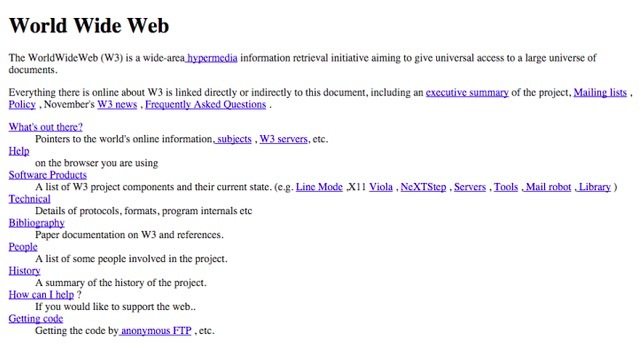
\includegraphics[width=80mm]{memoria/LaTeX/img/introduccion/web1.jpg}
    \caption[Ejemplo web 1º generación]{Ejemplo web 1º generación}
\end{figure}

\subsection{Las primeras app web (web 2.0)}

Debido a las limitaciones que ofrece la web 1.0, nace una nueva forma de concebir la web donde se valora las reacciones de los usuarios. Surgen aplicaciones y páginas que utilizan la inteligencia colectiva, consecuencia de ello las páginas pueden ser personalizadas convirtiéndose en una herramienta dinámica que permite el intercambio de información. Es por eso que la información se transforma en comunicación gracias a la interacción y a la incorporación de textos, vídeos, chats… Con esta nueva forma de concebir la web nacen los blogs, las redes sociales, los wikis … Este cambio ha supuesto una gran revolución, puesto que permite devolver la información de los usuarios y poder procesarla con el objetivo de controlar mejor la demanda. 


\begin{figure}[H]
    \centering
    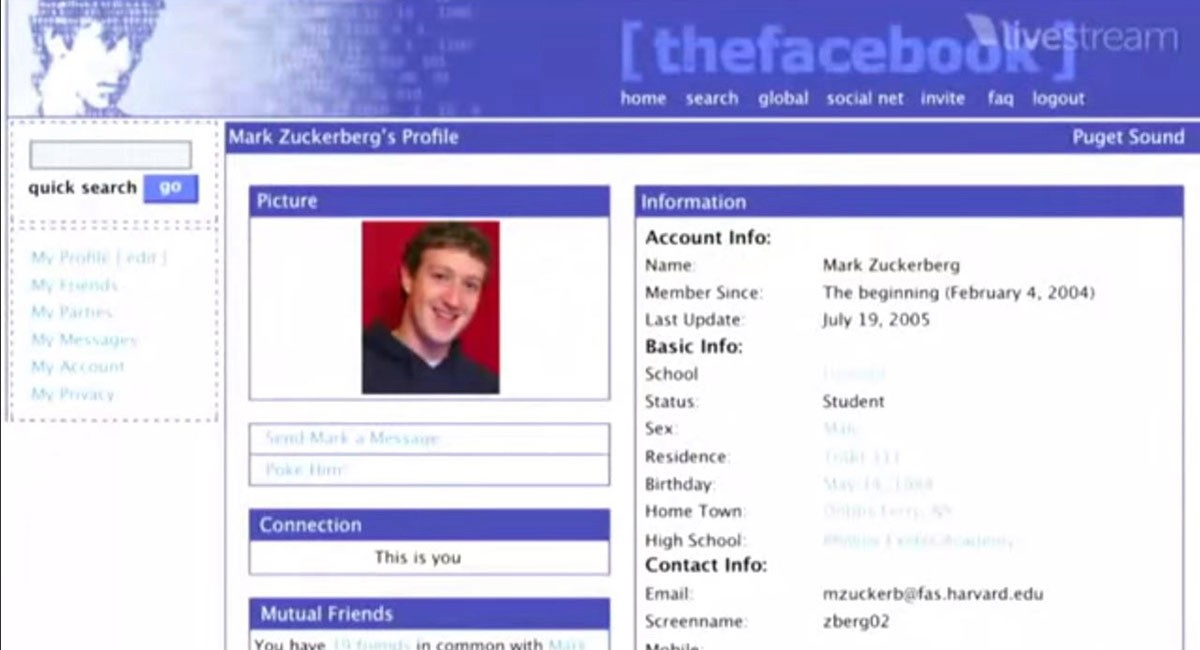
\includegraphics[width=80mm]{memoria/LaTeX/img/introduccion/web2.jpeg}
    \caption{Ejemplo web 2º generación}
\end{figure}
\subsection{Las app web de hoy en día}

La conocida web 3.0 dará paso a otro tipo de web donde pondrá su objetivo en la inteligencia artificial, un método para que los usuarios puedan no solo encontrar la información sino comprenderla. Este control esta en manos de motores informáticos y procesadores de información, que tratan de analizar nuestro perfil y nuestra actividad en red para enviarnos información de nuestro interés. 
Es por esto que la web 3.0 es definida por el concepto "personalización", ya que pretende devolver al usuario una información lo más afinada posible, filtrada a sus gustos y preferencias, evitando información que no sea de su interés.

\begin{figure}[H]
    \centering
    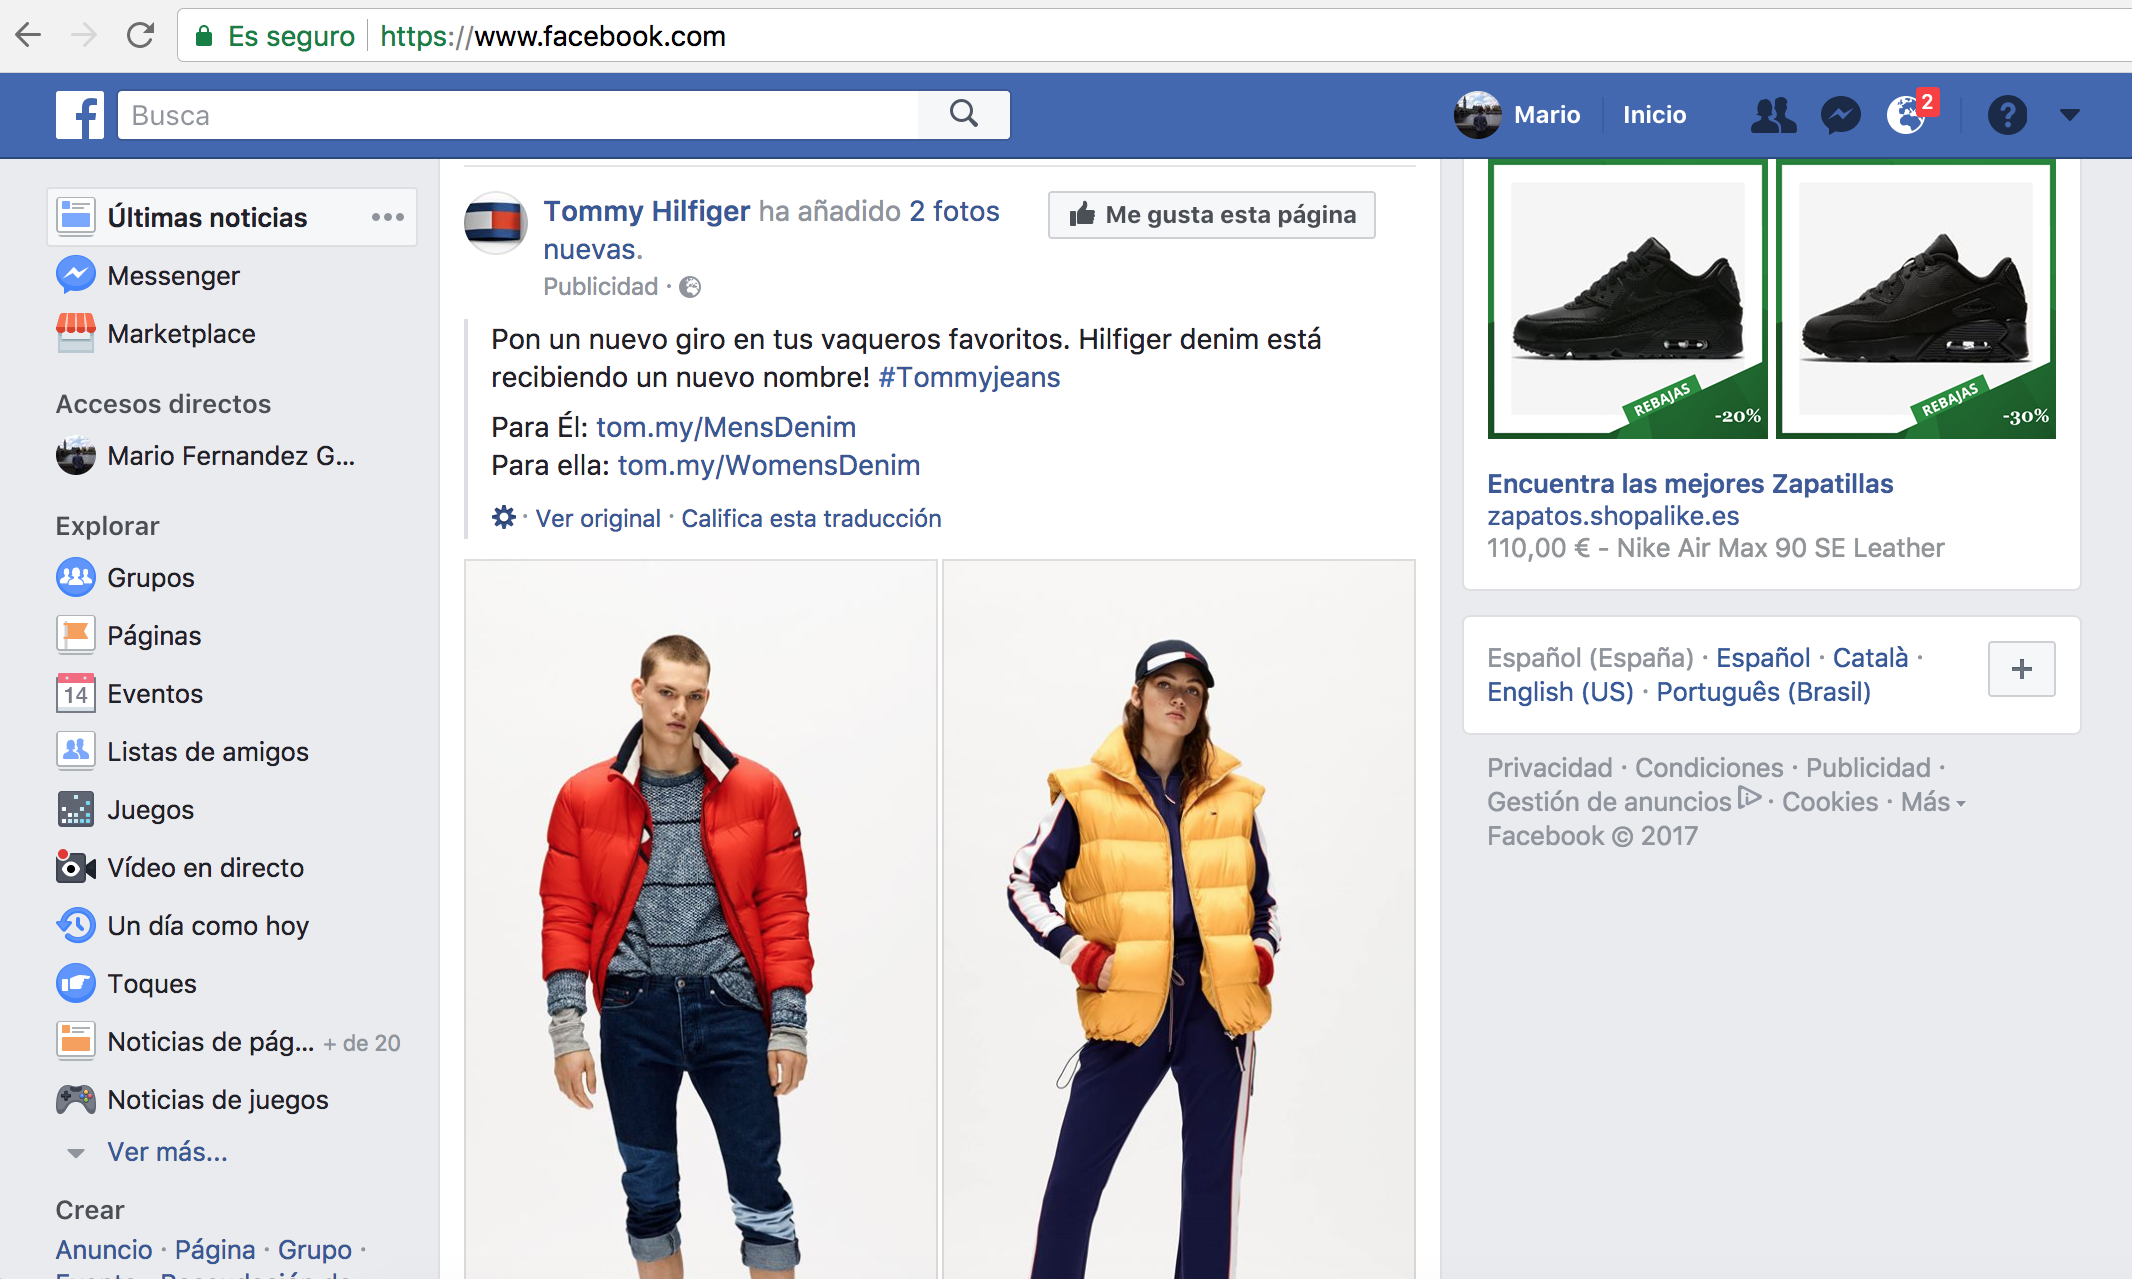
\includegraphics[width=80mm]{memoria/LaTeX/img/introduccion/facebook.png}
    \caption{Ejemplo web 3º generación}
\end{figure}

Con la aparición de la web 3.0, nuevos términos tecnológicos aparecen como:
\begin{itemize}
     \item \textbf{Web SPA: }Una web SPA es una aplicación de una sola página en la que la carga de datos es asíncrona y la página no se recarga en casi ningún momento, pese a cambiar de ruta o url para navegar entre las secciones de la aplicación, es una nueva tendencia en el desarrollo web.
     \item \textbf{Big Data: } Big data o macrodatos es un término que hace referencia a una cantidad de datos tal que supera la capacidad del software convencional para ser capturados, administrados y procesados en un tiempo razonable. El volumen de los datos masivos crece constantemente. En 2012 se estimaba su tamaño de entre una docena de terabytes hasta varios petabytes de datos en un único conjunto de datos.
    \item \textbf{API REST: } El término sirve para describir cualquier interfaz entre sistemas que utilice directamente HTTP para obtener datos o indicar la ejecución de operaciones sobre los datos, en cualquier formato(XML, JSON, etc).
    \begin{figure}[H]
    \centering
    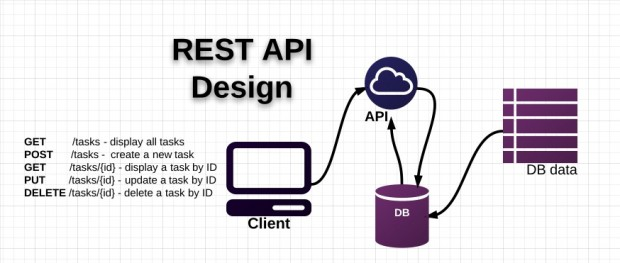
\includegraphics[width=90mm]{memoria/LaTeX/img/introduccion/rest-api.jpg}
    \caption{API-REST}
    \end{figure}
\end{itemize}

\section{Classcity}
\subsection{Objetivo}

Classcity consiste en una aplicación web desarrollada con tecnología de última  generación, cuyo objetivo principal es facilitar el contacto entre alumnos y profesores para dar clases particulares. Classcity utiliza la geolocalización del alumno para proporcionarle los profesores más próximos a él, además de poder filtrar por diferentes parámetros como curso, asignatura y distancia.

\begin{figure}[H]
    \centering
    
\includegraphics[width=40mm]{memoria/LaTeX/img/introduccion/logo.jpg}
\end{figure}

\subsection{Motivación}

Classcity nace motivada por la gran demanda de alumnos que se encuentran con la necesidad de poder encontrar un profesor bien referenciado y que se encuentre próximo al alumno. Es por esto por lo que surge Classcity, una nueva forma de encontrar a tu profesor particular donde el alumno es quien se encarga de buscar al profesor que mas se adapte a sus necesidades.

\subsection{Modelo de negocio}

Aunque no es algo que se haya tenido en cuenta en la implementación del código, Classcity podría tener un modelo de negocio claro.
Cada vez que un alumno concierte una clase con un profesor, se procederá a tramitar el coste de la clase por la aplicación suponiendo que un porcentaje del coste total de la clase vaya destinado al mantenimiento de classcity.
Por otro lado también se podría cobrar a los profesores por una mejor posición en nuestra aplicación, algo así como una cuenta cuenta premium de profesores donde tenga ciertas ventajas sobre las cuentas normales.

\section{Aplicaciones con éxito}


Classcity ha sido desarrollada basándose en modelos de aplicaciones que hoy en día están funcionando, como por ejemplo:

\subsection{Airbnb}

Es una empresa y una plataforma de software dedicada a la oferta de alojamientos a particulares y turísticos. El nombre es un acrónimo de airbed and breakfast (colchón inflable y desayuno). Airbnb tiene una oferta de unas 2.000.000 propiedades en 192 países y 33.000 ciudades. Desde su creación en noviembre de 2008 hasta junio de 2012 se realizaron 10 millones de reservas.

\begin{figure}[H]
    \centering
    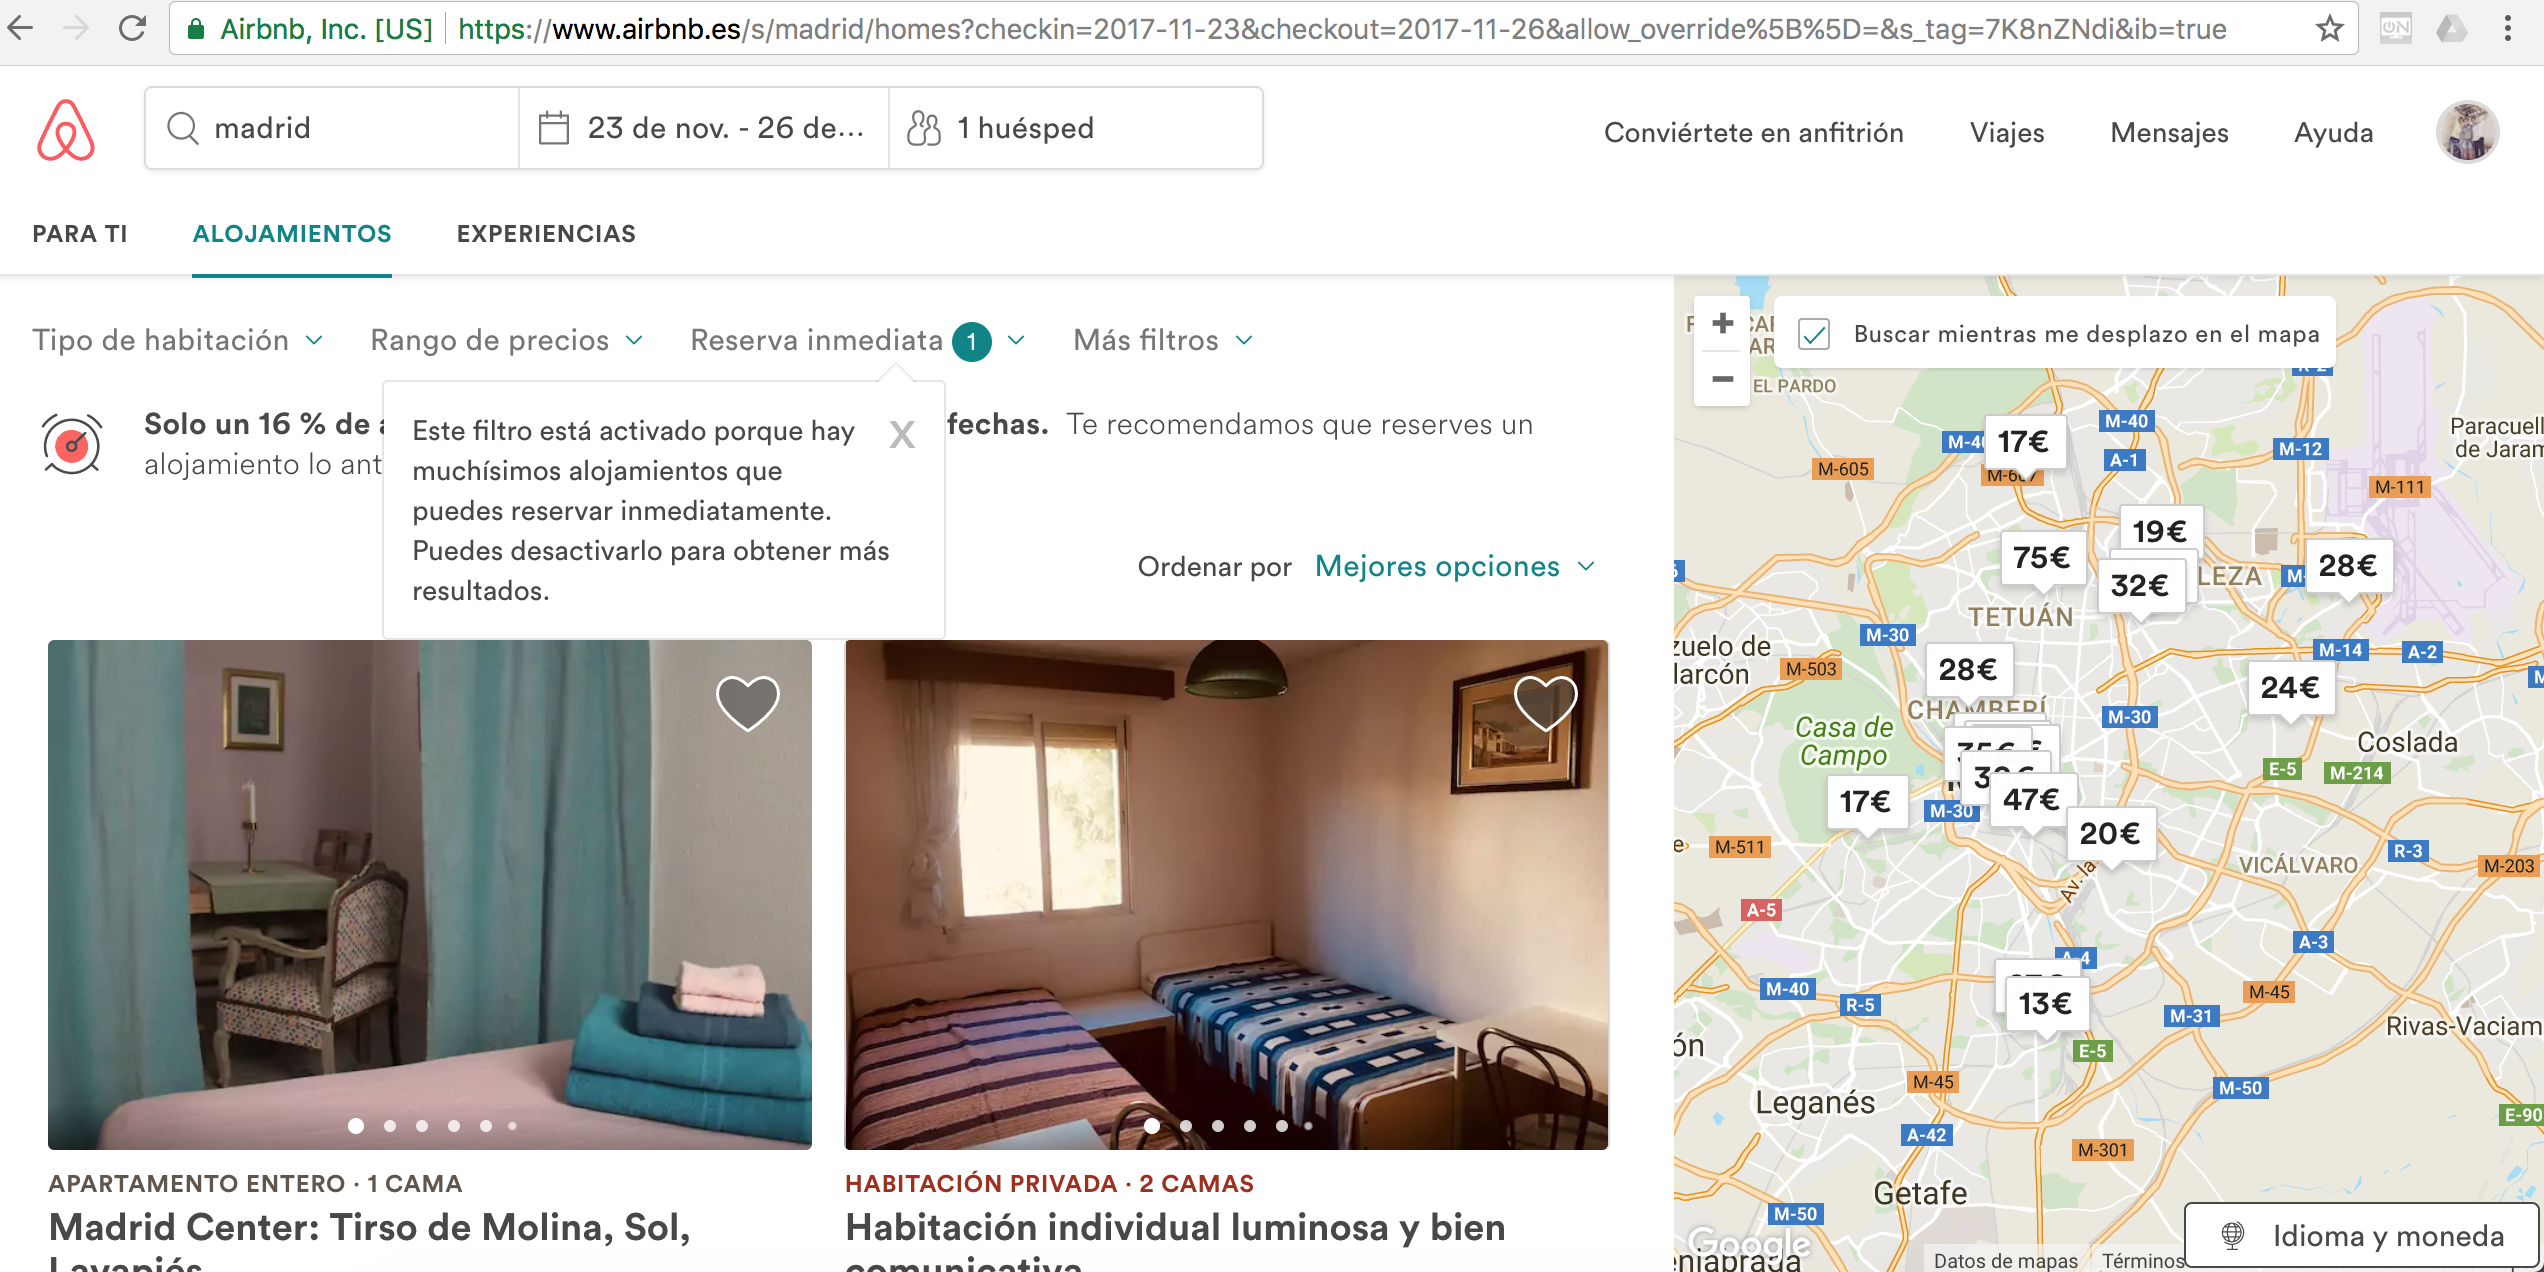
\includegraphics[width=100mm]{memoria/LaTeX/img/introduccion/airbnb.png}
    \caption{Aplicación Airbnb}
\end{figure}

\subsection{Blablacar}

Es un servicio de vehículo compartido que hace posible que las personas que quieren desplazarse al mismo lugar al mismo momento puedan organizarse para viajar juntos. Permite compartir los gastos puntuales del viaje (combustible y peajes) y también evitar la emisión extra de gases de efecto invernadero, al permitir una mayor eficiencia energética en el uso de cada vehículo.

\begin{figure}[H]
    \centering
    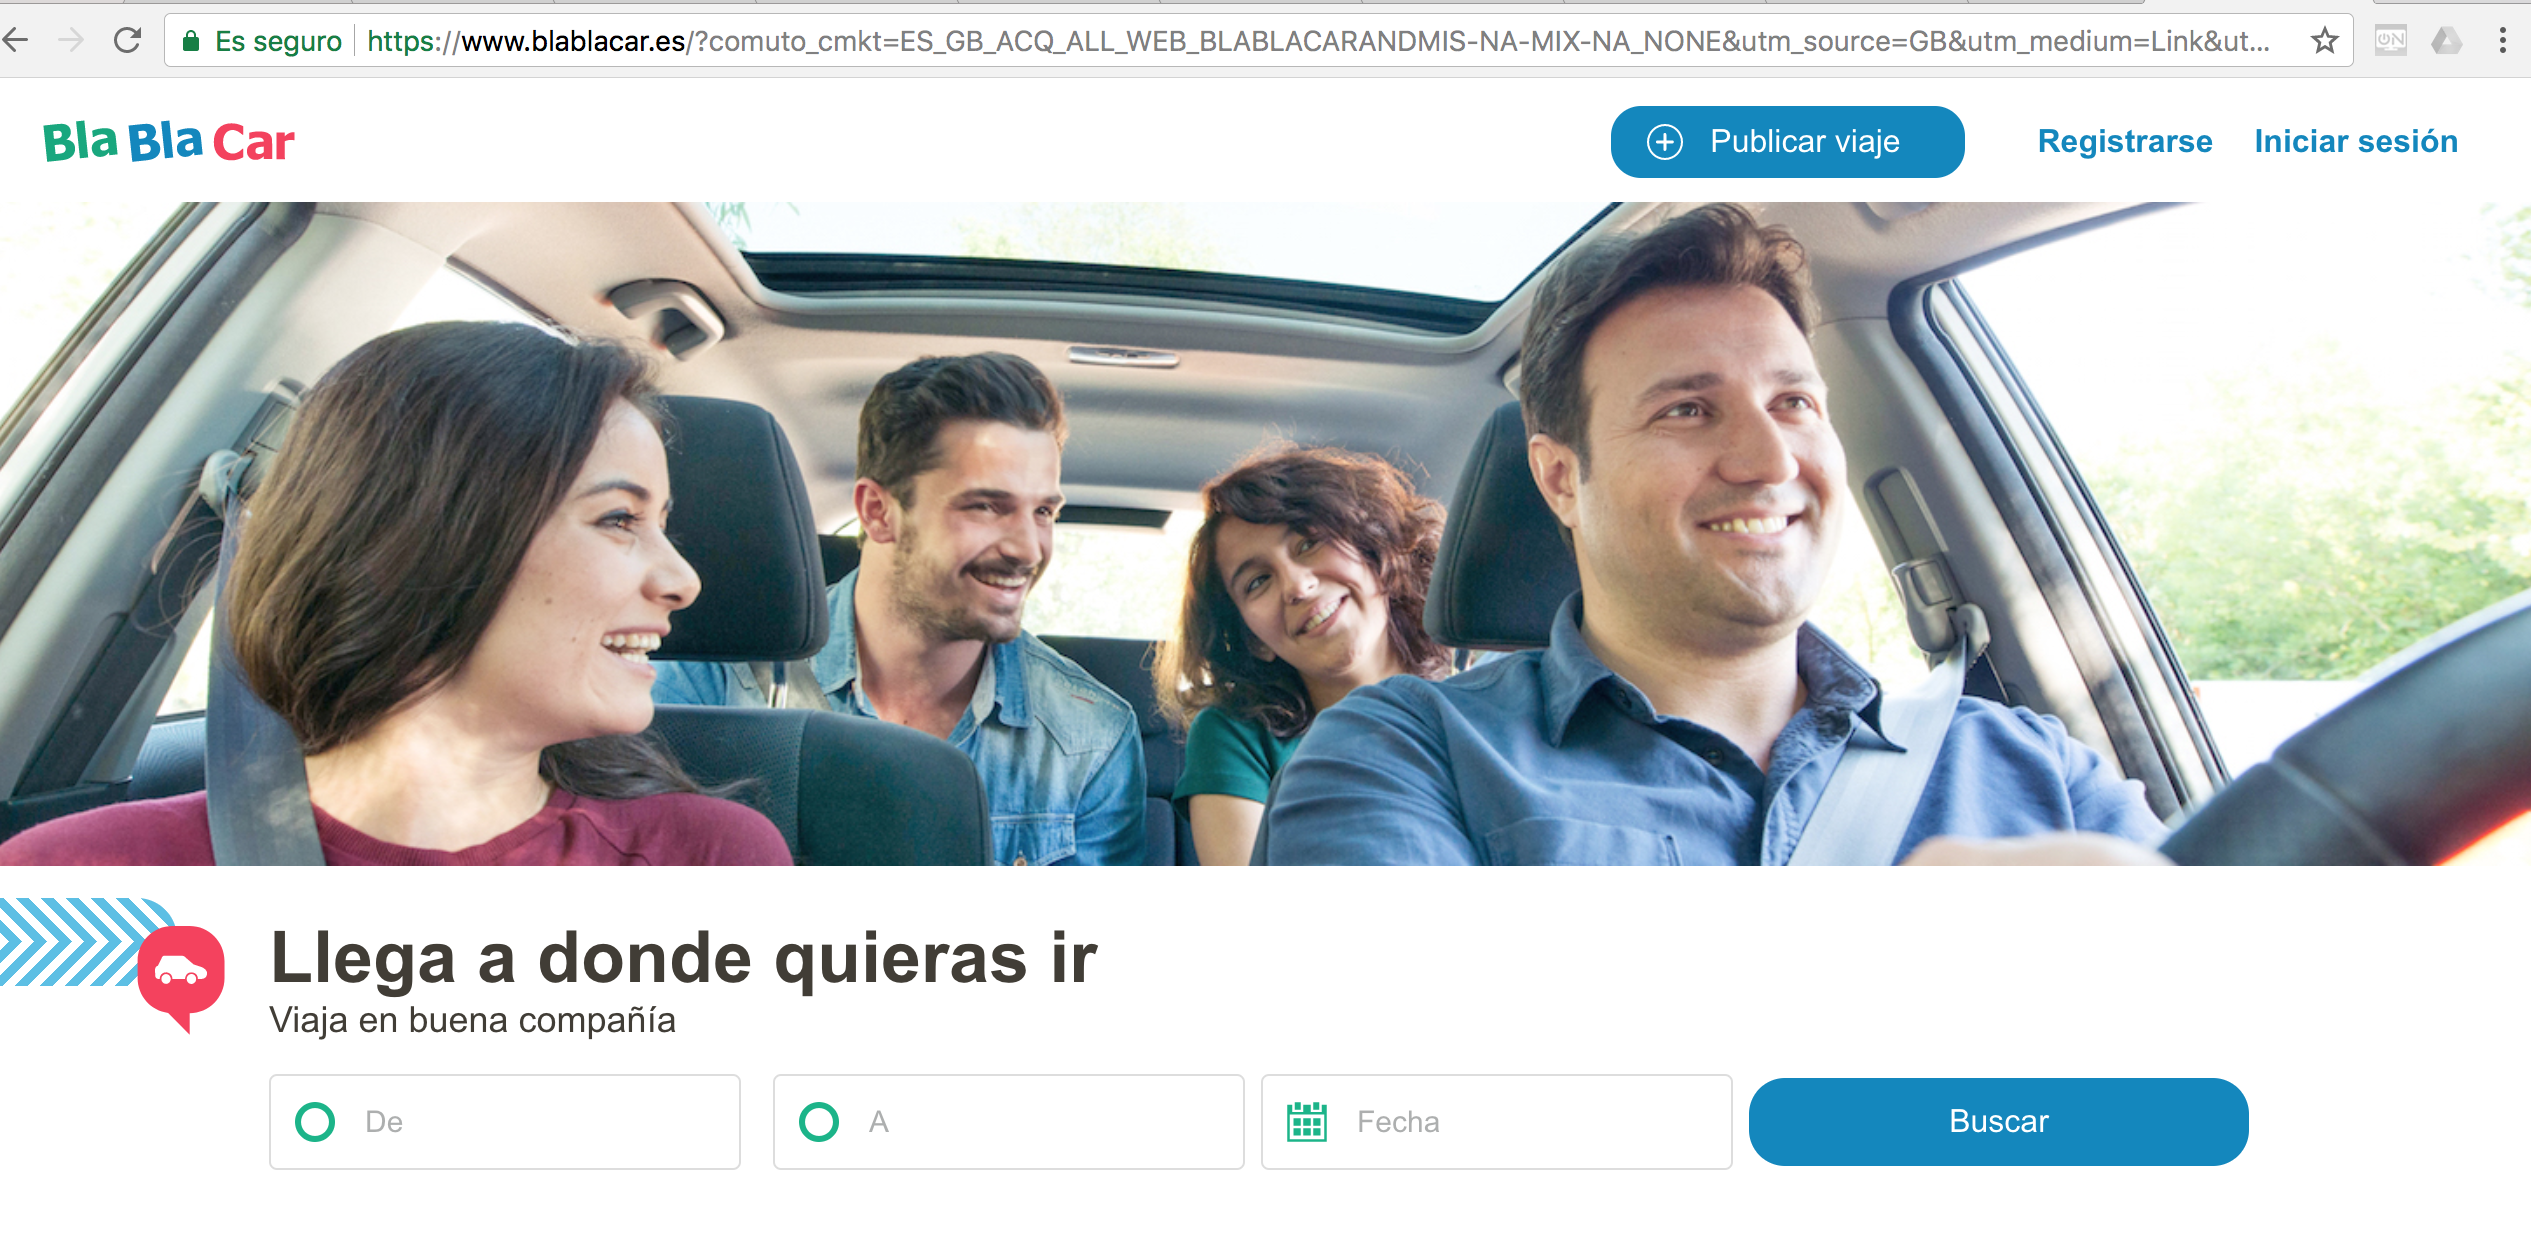
\includegraphics[width=120mm]{memoria/LaTeX/img/introduccion/blablacar.png}
    \caption{Aplicación Blablacar}
\end{figure}

\subsection{Wallapop}

Es una empresa española fundada en 2013, que ofrece un website dedicado a la compra y venta de productos de segunda mano entre usuarios a través de Internet, con un uso centrado en smartphones. Utiliza la geolocalización para que los usuarios puedan comprar y vender en función de su proximidad geográfica

\begin{figure}[H]
    \centering
    
\includegraphics[width=80mm]{memoria/LaTeX/img/introduccion/Wallapop-iPhone.jpg}
    \caption{Aplicación Wallapop}
\end{figure}


\section{Aplicaciones web realizadas en la URJC}

Este TFG centra su desarrollo en técnologias web, es por eso que tanto los proyectos de Edgar Barrero como de Pablo Parejo me han servido para tener una estructura solida de como encaminar mi aplicación web.

\subsection{Suveillance 5.1}

Edgar barrero desarrollo en Ruby sobre Rails Suveillance 5.1, una aplicación web que ofrece un flujo de vídeo desde una cámara web, un flujo de imagen de profundidad procedente de un sector Kinect y su representación en 3D, además de un sensor de humedad y un actuador. 


\begin{figure}[H]
    \centering
    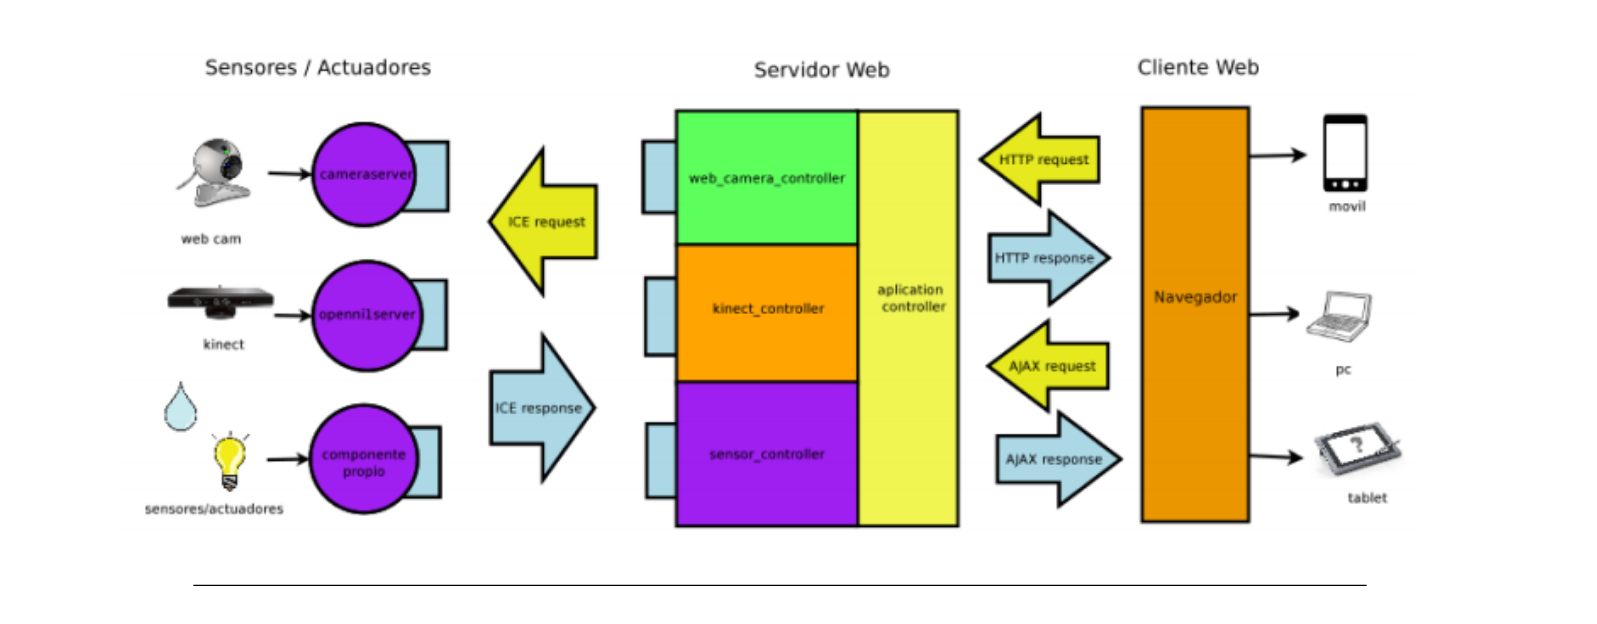
\includegraphics[width=110mm]{memoria/LaTeX/img/introduccion/edgar.png}
    \caption{TFG Edgar Barrero}
\end{figure}

\subsection{Gestión de servicios}
Pablo Parejo desarrollo una aplicación web donde poder gestionar de manera única todos los servicios de almacenamiento en línea que pueda tener un usuario. Aprovechando la oportunidad para adentrarse en tecnologías de última generación como: Angular, CSS3, HTML5, Django...
\begin{figure}[H]
    \centering
    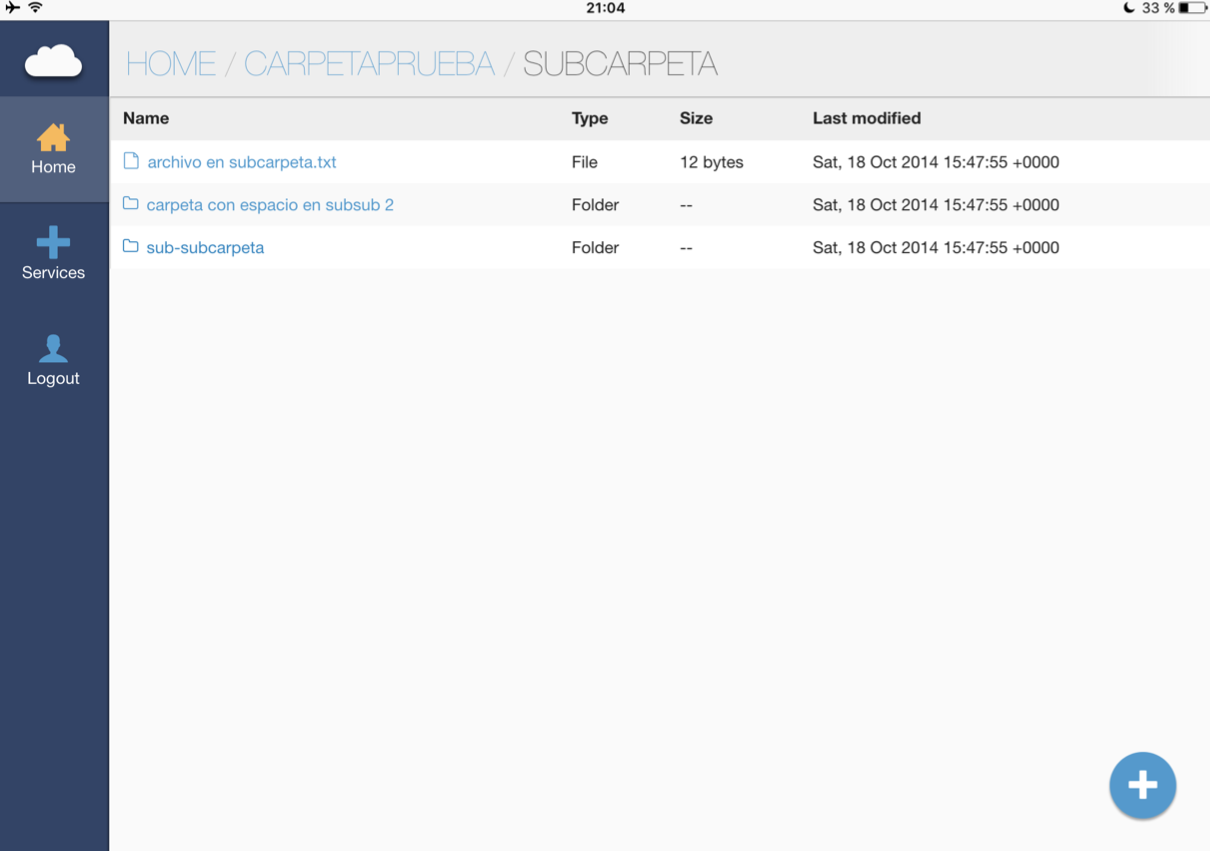
\includegraphics[width=90mm]{memoria/LaTeX/img/introduccion/parejo.png}
    \caption{TFG Pablo Parejo}
\end{figure}














































































































